\section{Vulnerability: JavaScript Injection Attack}
\label{sec:background}
\textbf{Description:} A second type of injection attack works on this website. It was possible to enter a JavaScript script into the transaction box. This would be stored by
the database as the description of the transaction. Consequently when the user clicked \textit{List transactions} each transaction would be listed, and as such each description
interpreted in html. This means a description enclosed by \verb|<script></script>| tags will be interpreted as a script and as such executed as the website comes to list the
transactions. This allows a hacker to gain valuable information by printing out session data in a pop up window. This security flaw is exasperated by the fact that all transactions
are viewable to all users. Thus any script injected will affect all users. This is known as a persistent (or stored) vulnerability. Persistent vulnerabilities are more significant
since the malicious script is rendered automatically, therefore there is no requirement to individually target victims or to take them to a third party website.\\ \\
\textbf{Testing the Vulnerability:} To test this vulnerability a series of JavaScript queries were entered as transactions. One of the most dangerous was the following:
\begin{minted}{html}
<script>alert(document.cookie)</script>
\end{minted}
Once injected upon the selection of \textit{List transactions} this will open a popup window which will display the user's token.
\begin{figure}[h]
  \centering
  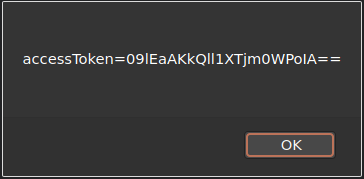
\includegraphics[width=0.5\textwidth]{figs/popup.png}
  \caption{The popup window displayed when a user clicks \textit{List transactions}}
  \label{popup}
\end{figure}\\
As can be seen from this figure, this injection allows a user to display the token. This again being particularly dangerous since the tokens are not time dependent on this website.
Consequently this can be said to be a major security flaw since it has the possibility of allowing a hacker indefinite access to the banking website.\\ \\
\textbf{Mitigation:} This vulnerability needs to be addressed with the use of \textit{html encoding}. This interprets certain key symbols such as < and > such that the website knows
they are simply to be printed and not interpreted as that symbol. As such they need to be stored differently, for example in our example < is stored as \verb|&lt;| and > is stored as
\verb|&gt;| Then when the website encounters these new encodings it knows to print < and > rather than when it encounters < and > which means the start of something such as a
script. In order to ensure the most rigorous security I imported a library to perform this encoding:
\begin{minted}{java}
import org.apache.commons.lang.StringEscapeUtils;
\end{minted}
From there the \verb|escapeHtml()| function was used to generate a new html encoded description of the transaction in the \verb|createTransaction()| function, which was then
entered into the database in place of the description.
\begin{minted}{java}
String encoded = StringEscapeUtils.escapeHtml(description);
\end{minted}
This works as required and if you look at the database you'll see the encoded raw text.
\begin{figure}[h]
  \centering
  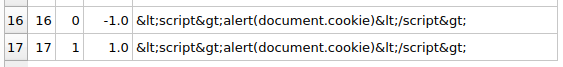
\includegraphics[width=0.8\textwidth]{figs/database.png}
  \caption{The transaction description as stored by the database}
  \label{fig2}
\end{figure}\\
Whilst the website correctly interprets this, printing < > rather than \verb|&lt;| \verb|&gt;|
\begin{figure}[h]
  \centering
  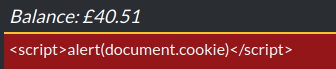
\includegraphics[width=0.5\textwidth]{figs/websitejs.png}
  \caption{The transaction description as interpreted by the browser}
  \label{fig3}
\end{figure}\\
This difference between the string stored by the database compared to the string entered by the user is what has been used to develop an automated test. The test enters a new
transaction containing the tags \verb|<script>| and \verb|</script>|. Then it checks to ensure that the value stored by the database does not contain either < or >. It also
checks to see if the transaction contains &lt; and &gt; to make sure the process works. Which by
ensuring, it can confirm that the threat of JavaScript injection is no longer a concern. See \verb|test3.java| for the full test.